\documentclass[12pt,a4paper,twoside]{article}  % Cambié "twosite" por "twoside"
\usepackage[utf8]{inputenc}  % Soporte para UTF-8
\usepackage[T1]{fontenc}     % Codificación de salida correcta
\usepackage[spanish]{babel}  % Paquete para el idioma español
\usepackage{graphicx}
\usepackage{grffile}
\usepackage{longtable}
\usepackage{wrapfig}
\usepackage{rotating}
\usepackage[normalem]{ulem}
\usepackage{amsmath}
\usepackage{textcomp}
\usepackage{amssymb}
\usepackage{capt-of}
\usepackage{hyperref}
\usepackage[left=2.00cm, right=2.50cm, top=2.50cm, bottom=2.00cm]{geometry}
\usepackage{fancyhdr}
\usepackage{listings}
\usepackage{xcolor}
\usepackage{float}
\usepackage[utf8]{inputenc}


% Configuración de listings para código MATLAB
\lstset{
    language=Matlab,
    basicstyle=\ttfamily\small,
    keywordstyle=\color{blue},
    commentstyle=\color{green},
    stringstyle=\color{red},
    stepnumber=1,
    breaklines=true,
    frame=single,
    tabsize=4,
    showspaces=false,
    showstringspaces=false
}

\hypersetup{
    pdfauthor={},
    pdftitle={IEEE-830},
    pdfkeywords={},
    pdfsubject={},
    pdfcreator={Emacs 26.2 (Org mode 9.1.9)},
    pdflang={English}
}

\begin{document}

% Portada
\begin{titlepage}
  \centering
  
\includegraphics[width=0.3\textwidth]{unsa-logo.png}\par\vspace{1cm}
  {\scshape\LARGE Universidad Nacional de San Agustín \par}
  {\scshape\Large Facultad de Ingeniería de Producción y Servicios\par}
  {\scshape\large Escuela Profesional de Ingeniería en Telecomunicaciones \par}
  \vspace{0.5cm}
  {\Large\bfseries Curso \par}
  {\Large\bfseries Métodos Numéricos  \par}
  \vspace{0.5cm}
  {\Large\itshape Doc: Edwing Alexander Gonzales Quilca \par}
  \vspace{0.5cm}
  {\Large\bfseries Solución de ejercicios \par}
  \vspace{0.5cm}
  {\Large Método de Newton y Secante\par}

  \vspace{2cm}

  Elaborado por\par
  {\Large\itshape Darwin Cristhian Turpo Quispe \par}
  {\Large\itshape Vladimir Williams Luque Llanqui \par}
  {\Large\itshape Luis Eduardo Pari Acuña \par}
  
\end{titlepage}



\newpage
\tableofcontents




\newpage
\section{Introducción:}

Este documento presenta la resolución de diversos ejercicios mediante la aplicación de métodos numéricos en MATLAB, como los métodos de Newton, Secante, Bisección, Regla Falsa, Punto Fijo, Eliminación Gaussiana, Factorización LU, Jacobi, y Gauss-Seidel. Estas técnicas son esenciales en ingeniería y ciencias aplicadas, ya que permiten encontrar raíces de funciones no lineales, resolver sistemas de ecuaciones y aproximar soluciones con gran precisión.

El Método de Newton o Newton-Raphson es un algoritmo iterativo conocido por su rapidez de convergencia en aproximaciones sucesivas a las raíces de funciones reales, especialmente cuando la solución inicial se encuentra cercana a la raíz buscada. En contraste, el Método de la Secante, una variación del método de Newton, no requiere el cálculo de la derivada de la función, lo que lo hace adecuado en situaciones donde la derivada no está disponible o es complicada de obtener.

Este documento también explora aplicaciones prácticas en telecomunicaciones, como el cálculo de atenuación óptima en fibras ópticas para minimizar la pérdida de señal, utilizando técnicas como la Bisección y la Regla Falsa. A lo largo de los ejercicios, se detallan los pasos de cada método, los resultados obtenidos, y se presentan gráficos y tablas que ilustran el comportamiento de las funciones y la convergencia de los métodos, con un análisis de sus ventajas y limitaciones.



\newpage

\section{Método de la Bisección:}

\textbf{a) Ejercicio 1: }

En telecomunicaciones, uno de los problemas comunes es calcular la atenuación óptima en una fibra óptica para minimizar la pérdida de señal. Imagina que tienes un sistema de comunicación por fibra óptica y necesitas encontrar el valor óptimo de potencia de señal en una sección de la fibra. La función de pérdida de señal en función de la potencia de entrada \(X\) está dada por \(f(X) = 0.5X^3 - 3X^2 + 4X - 2\). Encuentra el valor de \(X\) en el intervalo \([0, 5]\) que minimiza la función de pérdida de señal. Usa el método de bisección con una tolerancia de \( \text{tol} = 0.001 \).


\textbf{b) Código Matlab:}

\begin{lstlisting}
a = input("Ingrese el valor de a= ");
b = input("Ingrese el valor de b= ");
tol = input("Ingrese el valor de tol= ");
f = input("Ingrese la funcion f=", 's');
f = inline(f);  
k = 1;          
m = (a + b) / 2; 

fprintf('k\tak\t\tbk\t\tmk\t\terror\n');

fa = f(a);
fm = f(m);

while (b - a) / 2 > tol
    fprintf('%d\t%f\t%f\t%f\t%f\n', k, a, b, m, (b - a) / 2);
    
    if fa * fm < 0  
        b = m;      
    else
        a = m;      
        fa = fm;    
    end
    
    m = (a + b) / 2;
    fm = f(m); 
    k = k + 1;  
end
fprintf('La raiz aproximada es m = %f\n', m);

\end{lstlisting}

\textbf{C) Salida:}

\begin{verbatim}
>> M_biseccion
Ingrese el valor de a= 
0
Ingrese el valor de b= 
5
Ingrese el valor de tol= 
0.001
Ingrese la funcion f=
0.5*x^3 - 3*x^2 + 4*x - 2
k	  ak		    bk	    	mk		     error
1	0.000000	5.000000	2.500000	2.500000
2	2.500000	5.000000	3.750000	1.250000
3	3.750000	5.000000	4.375000	0.625000
4	4.375000	5.000000	4.687500	0.312500
5	4.375000	4.687500	4.531250	0.156250
6	4.375000	4.531250	4.453125	0.078125
7	4.375000	4.453125	4.414062	0.039062
8	4.375000	4.414062	4.394531	0.019531
9	4.375000	4.394531	4.384766	0.009766
10	4.375000	4.384766	4.379883	0.004883
11	4.379883	4.384766	4.382324	0.002441
12	4.382324	4.384766	4.383545	0.001221
La raiz aproximada es m = 4.382935
>> 
\end{verbatim}

\textbf{d) Interpretación:}

El resultado \( m = 4.382935 \) indica que, con una precisión de 0.001, el valor de \( X \) que minimiza la pérdida de señal se encuentra aproximadamente en 4.38. Este valor de potencia es el óptimo dentro del intervalo \([0,5]\), según el método de bisección aplicado a la función de pérdida, y proporciona una configuración eficiente para reducir la atenuación de la señal en la fibra óptica. Este dato puede ser utilizado para ajustar la potencia de entrada en el sistema, optimizando así la transmisión en la fibra óptica.

% metodo----------------------------------------------------
\section{Método de la regla falsa:}

\textbf{a) Ejercicio 2: }

%pegar ejercicio n
Un ingeniero de telecomunicaciones necesita determinar el valor óptimo de un parámetro \( x \), que podría representar la resistencia en un circuito de transmisión, para maximizar la potencia de salida sin causar distorsión. La potencia de salida \( P(x) \) depende del parámetro \( x \) de acuerdo con una función no lineal \( f(x) = 100 - 0.01 \cdot x^2 \), donde 100 es el valor máximo de potencia deseada y \( 0.01 \) es una constante de ajuste basada en el diseño del circuito. Utilizando el método de Falsa Posición en el intervalo inicial \([a, b] = [10, 500]\) con una tolerancia de \( \text{tol} = 10^{-5} \) y un máximo de 100 iteraciones, determine el valor de \( x \) que hace que \( f(x) = 0 \), lo cual representa el punto de máxima eficiencia para la potencia en el circuito de transmisión.


\textbf{b) Código Matlab:}

\begin{lstlisting}
a = input("Ingrese el valor de a= ");
b = input("Ingrese el valor de b= ");
tol = input("Ingrese el valor de tol= ");
itera = input("Ingrese iteraciones = ");
f = input("Ingrese la funcion f=", 's');
f = inline(f);

k = 0; 
an = a;
bn = b;
fprintf('k\tan\t\tbn\t\txn\t\terror\n');

while true

    xn = an * f(bn) - bn * f(an);
    xn = xn / (f(bn) - f(an));
    
    e1 = abs(xn - an);
    e2 = abs(bn - xn);
    
    fprintf('%d\t%f\t%f\t%f\t%f\n', k, an, bn, xn, max(e1, e2));
    
    if max(e1, e2) <= tol || k >= itera
        break;
    end
    
    if f(xn) * f(an) > 0
        an = xn;
    else
        bn = xn;
    end
    
    k = k + 1;
end

fprintf('La raiz aproximada es xn = %f\n', xn);

\end{lstlisting}

\textbf{c) Salida:}

\begin{verbatim}
>> Regla_falsa
Ingrese el valor de a= 
10
Ingrese el valor de b= 
500
Ingrese el valor de tol= 
1e-5
Ingrese iteraciones = 
20
Ingrese la función f=
100 - 0.01 * x^2
k	an		bn		xn		error
0	10.000000	500.000000	29.411765	470.588235
1	29.411765	500.000000	46.666667	453.333333
2	46.666667	500.000000	60.975610	439.024390
3	60.975610	500.000000	72.173913	427.826087
4	72.173913	500.000000	80.547112	419.452888
5	80.547112	500.000000	86.596859	413.403141
6	86.596859	500.000000	90.860407	409.139593
7	90.860407	500.000000	93.812689	406.187311
8	93.812689	500.000000	95.832146	404.167854
9	95.832146	500.000000	97.201995	402.798005
10	97.201995	500.000000	98.125924	401.874076
11	98.125924	500.000000	98.746701	401.253299
12	98.746701	500.000000	99.162718	400.837282
13	99.162718	500.000000	99.441032	400.558968
14	99.441032	500.000000	99.627007	400.372993
15	99.627007	500.000000	99.751184	400.248816
16	99.751184	500.000000	99.834054	400.165946
17	99.834054	500.000000	99.889338	400.110662
18	99.889338	500.000000	99.926212	400.073788
19	99.926212	500.000000	99.950802	400.049198
20	99.950802	500.000000	99.967199	400.032801
La raíz aproximada es xn = 99.967199
>>  

\end{verbatim}

\textbf{d) Interpretación:}

El valor encontrado, \( x = 99.967199 \), representa el punto donde la potencia de salida es máxima con eficiencia en el circuito. Este valor es óptimo dentro del intervalo \([10,500]\) y permite obtener la potencia de salida sin causar distorsión en el sistema. Este resultado es esencial para diseñar el circuito de transmisión con los valores de resistencia adecuados, garantizando el máximo rendimiento de potencia sin afectar la calidad de la señal.



\section{Método Newton}

\textbf{a) Ejercicio 3: }

%pegar ejercicio n
En telecomunicaciones, la ecuación de Friis para la transmisión de radiofrecuencia (RF) en espacio libre se puede simplificar para encontrar la distancia óptima de transmisión, utilizando métodos numéricos como Newton-Raphson. Queremos encontrar la distancia \( d \) que satisface la ecuación \( f(d) = \log(d) + d - 5 = 0 \), donde \( P_t/P_r = 5 \). El método iterativo se inicia con un valor inicial \( d_0 = 2 \) y una tolerancia de \( 1 \times 10^{-6} \). La derivada de la función es \( f'(d) = \frac{1}{d} + 1 \). Usamos el método de Newton-Raphson para aproximar la solución con el siguiente esquema: 
\[
d_{n+1} = d_n - \frac{f(d_n)}{f'(d_n)}
\]
hasta que la diferencia entre iteraciones consecutivas sea menor que la tolerancia especificada.


\textbf{b) Código Matlab:}

\begin{lstlisting}

x0=input('ingrese el valor inicial x= ');
tolerancia=input('ingrese la tolerancia tolerancia x= ');
f=input('ingrese la funcion f= ','s');
f=inline(f);
df=input('ingrese la derivada de la funcion f= ','s');
df=inline(df);
x1=x0-f(x0)/df(x0);
k=1
fprintf('k       xk      error\n')
while abs(x1-x0) > tolerancia
    fprintf('%d\t%.10f\t%.10f\n', k ,x1, abs(x1-x0))
    k=k+1;
    x0=x1;
    x1=x0-f(x0)/df(x0);
end
fprintf('%d\t%.10f\t%.10f\n', k ,x1, abs(x1-x0))

\end{lstlisting}

\textbf{c) Salida:}

\begin{verbatim}

>> M_Newton
ingrese el valor inicial x= 
2
ingrese la tolerancia tolerancia x= 
1e-6
ingrese la funcion f= 
log(d) + d - 5
ingrese la derivada de la funcion f= 
1/d + 1
k       xk      error
1	3.5379018796	1.5379018796
2	3.6927092953	0.1548074157
3	3.6934413435	0.0007320482
4	3.6934413590	0.0000000155
>> 

\end{verbatim}

\textbf{d) Interpretación:}

La solución aproximada obtenida es \( d = 3.6934413590 \). Esto significa que la distancia óptima de transmisión en espacio libre que maximiza la eficiencia en la transmisión de la señal es aproximadamente de 3.69 unidades. Este valor es crítico para ajustar la configuración del sistema de radiofrecuencia en telecomunicaciones, asegurando una transmisión efectiva y eficiente. La rapidez de convergencia del método Newton-Raphson también permite confirmar la precisión del valor obtenido dentro de la tolerancia especificada.



% metodo
\section{Método de la secante: }

\textbf{a) Ejercicio 4: }

%pegar ejercicio n
En telecomunicaciones, la ecuación de propagación de una onda electromagnética en espacio libre puede modelarse como \( f(d) = e^d - 4d = 0 \), donde \( d \) es la distancia entre las antenas. Se desea encontrar el valor de \( d \) que minimice la diferencia de potencia entre transmisor y receptor. Utilizando el método de la secante, con valores iniciales \( d_0 = 1.5 \) y \( d_1 = 2.5 \), y una tolerancia de \( 1 \times 10^{-6} \), se puede aplicar el siguiente esquema iterativo:
\[
d_{n+1} = d_n - f(d_n) \frac{d_n - d_{n-1}}{f(d_n) - f(d_{n-1})}
\]
hasta que la diferencia entre iteraciones consecutivas sea menor que la tolerancia especificada. El método secante no requiere el cálculo de la derivada, lo que lo hace más eficiente en ciertos casos donde la derivada de \( f \) es difícil de calcular.


\textbf{b) Código Matlab:}

\begin{lstlisting}

x0 = input('Ingrese el valor inicial x0= ');
x1 = input('Ingrese el valor inicial x1= ');
tolerancia = input('Ingrese la tolerancia tolerancia= ');
f = input('Ingrese la funcion f= ', 's');
f = inline(f);
k = 1;
fprintf('k       xk      error\n')
while abs(x1 - x0) > tolerancia
    x2 = x1 - f(x1) * (x1 - x0) / (f(x1) - f(x0));
    fprintf('%d\t%.10f\t%.10f\n', k, x2, abs(x2 - x1));
    x0 = x1;
    x1 = x2;
    k = k + 1;
end
fprintf('%d\t%.10f\t%.10f\n', k, x1, abs(x1 - x0));

\end{lstlisting}

\textbf{c) Salida:}

\begin{verbatim}

>> M_secante
Ingrese el valor inicial x0= 
1.5
Ingrese el valor inicial x1= 
2.5
Ingrese la tolerancia tolerancia= 
1e-6
Ingrese la funcion f= 
exp(d) - 4*d
k       xk      error
1	1.9102650571	0.5897349429
2	2.0805704847	0.1703054276
3	2.1736827679	0.0931122831
4	2.1518638029	0.0218189650
5	2.1532654775	0.0014016746
6	2.1532924000	0.0000269225
7	2.1532923641	0.0000000359
8	2.1532923641	0.0000000359
>> 

\end{verbatim}

\textbf{d) Interpretación:}

La distancia óptima aproximada entre antenas que minimiza la diferencia de potencia es 2.1533 unidades. Este resultado es crucial para optimizar la disposición de las antenas en el espacio, asegurando una transmisión eficiente sin pérdida de potencia significativa. La salida también demuestra la rapidez de convergencia del método de la secante, alcanzando una alta precisión en solo unas pocas iteraciones.


\section{Método del punto fijo: }

\textbf{a) Ejercicio 5: }

%pegar ejercicio n
\textbf{Problema:} En el campo de las telecomunicaciones, la ecuación que describe la propagación de una señal en espacio libre puede aproximarse mediante \( f(d) = \sqrt{d} + \log(d) - 3 = 0 \), donde \( d \) es la distancia entre las antenas. Para determinar el valor de \( d \) que minimiza la pérdida de señal, aplicamos un método iterativo comenzando con \( d_0 = 1.5 \) y una tolerancia de \( 1 \times 10^{-6} \). La relación iterativa está dada por:
\[
d_{n+1} = f(d_n)
\]
La iteración continúa hasta que el error absoluto \( |d_{n+1} - d_n| \) sea menor que la tolerancia, calculando también el error relativo en cada paso:
\[
\text{Error relativo} = \frac{|d_{n+1} - d_n|}{|d_{n+1}|}
\]
Este proceso iterativo es útil cuando la derivada de la función es difícil de obtener o no es necesaria.



\textbf{b) Código Matlab:}

\begin{lstlisting}

x0 = input('Ingrese el valor inicial x0= ');
tolerancia = input('Ingrese la tolerancia = ');
f = input('Ingrese la funcion f= ', 's');
f = inline(f);
x1 = f(x0);
k = 1;
fprintf('k         xk         error abs       error relativo\n')
while abs(x1 - x0) > tolerancia
    fprintf('%d\t%.10f\t%.10f\t%.10f\n', k, x1, abs(x1 - x0), ...
        abs(x1 - x0)/ abs(x1))
    k = k + 1;
    x0 = x1;
    x1 = f(x0);
end
 fprintf('%d\t%.10f\t%.10f\t%.10f\n', k, x1, abs(x1 - x0), ...
     abs(x1 - x0)/ abs(x1))

\end{lstlisting}

\textbf{c) Salida:}

\begin{verbatim}

>> M_puntofijo
Ingrese el valor inicial x0= 
1.5
Ingrese la tolerancia = 
1e-6
Ingrese la funcion f= 
sqrt(d) + log(d) - 3
k         xk         error abs       error relativo
1	-1.3697900205	2.8697900205	2.0950583502
2	-2.6853425416	4.5081913327	0.8874774944
3	-0.2805567042	2.4142680814	0.5877277547
4	-0.2037752451	0.9807940600	0.3136462846
5	-0.6509171510	0.4873752232	0.1625648959
6	-0.8187337645	0.2718471270	0.0837649201
7	-0.7212700220	0.1476739568	0.0443415956
8	-0.6547471748	0.0770697752	0.0235079310
9	-0.6672640050	0.0401949859	0.0123921203
10	-0.6883453663	0.0211900150	0.0065198259
11	-0.6895615026	0.0112000338	0.0034342994
12	-0.6839502645	0.0059054583	0.0018104650
13	-0.6823882653	0.0031098795	0.0009542759
14	-0.6836023090	0.0016383509	0.0005028596
15	-0.6843027167	0.0008634941	0.0002649804
16	-0.6841191928	0.0004550983	0.0001396402
17	-0.6838844108	0.0002398264	0.0000735894
18	-0.6838838785	0.0001263801	0.0000387805
19	-0.6839489605	0.0000665999	0.0000204366
20	-0.6839633867	0.0000350973	0.0000107697
21	-0.6839484773	0.0000184957	0.0000056755
22	-0.6839412003	0.0000097469	0.0000029909
23	-0.6839437443	0.0000051365	0.0000015761
24	-0.6839463234	0.0000027068	0.0000008306
25	-0.6839461826	0.0000014265	0.0000004377
26	-0.6839454355	0.0000007517	0.0000002307
>> 

\end{verbatim}

\textbf{d) Interpretación:}

El proceso de iteración indica que la distancia óptima aproximada es alrededor de -0.684 (sin embargo, este resultado es negativo, lo que puede indicar que el método o función requiere ajuste para la realidad física, ya que una distancia negativa no tiene sentido físico).

%%%%%%%%%%%%%%%%%%%%%%%%%%%%%%%%%%%%%%%%%%%%%%%%%%%%%%%%%%%%%%%%%%%%%%%%%%%%%%%%    
\section{Eliminación Gaussiana: }

\textbf{a) Ejercicio 6: }

Resolver el siguiente sistema de ecuaciones lineales utilizando el método de eliminación de Gauss con pivoteo parcial:

\[
\begin{aligned}
3x_1 + 2x_2 + 4x_3 &= 1 \\
2x_1 + 3x_2 + 3x_3 &= 2 \\
5x_1 + 4x_2 + 6x_3 &= 3
\end{aligned}
\]
Escribe la matriz aumentada correspondiente y aplica el algoritmo de eliminación de Gauss para encontrar los valores de \( x_1 \), \( x_2 \) y \( x_3 \).




\textbf{b) Código Matlab:}

\begin{lstlisting}

A = input('Ingrese la matriz aumentada A= ');
[n, m] = size(A);
for i = 1:n-1
    for p = i:n
        if A(p,i) ~= 0
            break
        else
            disp('xd')
        end
    end
    if p ~= i
        aux = A(i,:);
        A(i,:) = A(p,:);
        A(p,:) = aux;
    end
    for j = i+1:n
        M(j,i) = A(j,i)/A(i,i);
        A(j,:) = A(j,:) - M(j,i) * A(i,:)
    end
end
if A(n,n) == 0
    disp('No existe solucion unica');
else
    x(n) = A(n,n+1)/A(n,n);
    for i = n-1:-1:1
        sum = 0;
        for j = i+1:n
            sum = sum + A(i,j) * x(j);
        end
        x(i) = (A(i,n+1) - sum) / A(i,i);
    end
    
    for k = 1:n
        fprintf('x%d = %.4f\n', k, x(k));
    end
end


\end{lstlisting}

\textbf{c) Salida:}

\begin{verbatim}

>> M_Gaussiana
Ingrese la matriz aumentada A= 
[3 2 4 1 ; 2 3 3 2 ;5 4 6  3]

A =

    3.0000    2.0000    4.0000    1.0000
         0    1.6667    0.3333    1.3333
    5.0000    4.0000    6.0000    3.0000


A =

    3.0000    2.0000    4.0000    1.0000
         0    1.6667    0.3333    1.3333
         0    0.6667   -0.6667    1.3333


A =

    3.0000    2.0000    4.0000    1.0000
         0    1.6667    0.3333    1.3333
         0         0   -0.8000    0.8000

x1 = 1.0000
x2 = 1.0000
x3 = -1.0000
>> 

\end{verbatim}




%%%%%%%%%%%%%%%%%%%%%%%%%%%%%%%%%%%%%%%%%%%%%%%%%%%%%%%%%%%%%%%%%%%%%%%%%%%%%%%%
\section{Factorización LU: }

\textbf{a) Ejercicio 7: }

Resolver el siguiente sistema de ecuaciones lineales utilizando factorización LU:

\[
\begin{aligned}
2x_1 + 3x_2 - x_3 + 4x_4 + 5x_5 &= 15 \\
x_1 - 2x_2 + 3x_3 + x_4 - x_5 &= 3 \\
4x_1 + x_2 + 2x_3 -  3x_4 + x_5 &= 10 \\
-x_1 +  5x_2 + x_3 + 2x_4 - 2x_5 &= 1 \\
3x_1 - x_2 + 4x_3 + 2x_4 + x_5 &= 12
\end{aligned}
\]

Escribe la matriz aumentada correspondiente y aplica el algoritmo de factorización LU para descomponer la matriz en \( L \) y \( U \). Luego, resuelve el sistema utilizando sustitución hacia adelante y hacia atrás para encontrar los valores de \( x_1, x_2, x_3, x_4 \) y \( x_5 \).




\textbf{b) Código Matlab:}

\begin{lstlisting}

A = input('Ingrese la matriz aumentada A= ');
b = input('ingrese el lado derecho de b=');
[n,m]=size(A);
M=eye(n);
for i=1:n-1
    for j=i+1:n
        M(j,i)=A(j,i)/A(i,i);
        A(j,:)=A(j,:)-M(j,i)*A(i,:)
    end
end
L=M
U=A
y = zeros(n, 1);
for i = 1:n
    y(i) = b(i) - L(i, 1:i-1) * y(1:i-1);
end
x = zeros(n, 1);
for i = n:-1:1
    x(i) = (y(i) - U(i, i+1:n) * x(i+1:n)) / U(i, i); 
end

disp(x);

\end{lstlisting}

\textbf{c) Salida:}

\begin{verbatim}

>> M_LU
Ingrese la matriz aumentada A= 
[
    2, 3, -1, 4, 5;
    1, -2, 3, 1, -1;
    4, 1, 2, -3, 1;
    -1, 5, 1, 2, -2;
    3, -1, 4, 2, 1
]
ingrese el lado derecho de b=
[15; 3; 10; 1; 12]

A =

    2.0000    3.0000   -1.0000    4.0000    5.0000
         0   -3.5000    3.5000   -1.0000   -3.5000
    4.0000    1.0000    2.0000   -3.0000    1.0000
   -1.0000    5.0000    1.0000    2.0000   -2.0000
    3.0000   -1.0000    4.0000    2.0000    1.0000


A =

    2.0000    3.0000   -1.0000    4.0000    5.0000
         0   -3.5000    3.5000   -1.0000   -3.5000
         0   -5.0000    4.0000  -11.0000   -9.0000
   -1.0000    5.0000    1.0000    2.0000   -2.0000
    3.0000   -1.0000    4.0000    2.0000    1.0000


A =

    2.0000    3.0000   -1.0000    4.0000    5.0000
         0   -3.5000    3.5000   -1.0000   -3.5000
         0   -5.0000    4.0000  -11.0000   -9.0000
         0    6.5000    0.5000    4.0000    0.5000
    3.0000   -1.0000    4.0000    2.0000    1.0000


A =

    2.0000    3.0000   -1.0000    4.0000    5.0000
         0   -3.5000    3.5000   -1.0000   -3.5000
         0   -5.0000    4.0000  -11.0000   -9.0000
         0    6.5000    0.5000    4.0000    0.5000
         0   -5.5000    5.5000   -4.0000   -6.5000


A =

    2.0000    3.0000   -1.0000    4.0000    5.0000
         0   -3.5000    3.5000   -1.0000   -3.5000
         0         0   -1.0000   -9.5714   -4.0000
         0    6.5000    0.5000    4.0000    0.5000
         0   -5.5000    5.5000   -4.0000   -6.5000


A =

    2.0000    3.0000   -1.0000    4.0000    5.0000
         0   -3.5000    3.5000   -1.0000   -3.5000
         0         0   -1.0000   -9.5714   -4.0000
         0         0    7.0000    2.1429   -6.0000
         0   -5.5000    5.5000   -4.0000   -6.5000


A =

    2.0000    3.0000   -1.0000    4.0000    5.0000
         0   -3.5000    3.5000   -1.0000   -3.5000
         0         0   -1.0000   -9.5714   -4.0000
         0          0         0  -64.8571  -34.0000
         0         0         0   -2.4286   -1.0000


A =

    2.0000    3.0000   -1.0000    4.0000    5.0000
         0   -3.5000    3.5000   -1.0000   -3.5000
         0         0   -1.0000   -9.5714   -4.0000
         0         0         0  -64.8571  -34.0000
         0         0         0   -2.4286   -1.0000


A =

    2.0000    3.0000   -1.0000    4.0000    5.0000
         0   -3.5000    3.5000   -1.0000   -3.5000
         0         0   -1.0000   -9.5714   -4.0000
         0         0         0  -64.8571  -34.0000
         0         0         0         0    0.2731


L =

    1.0000         0         0         0         0
    0.5000    1.0000         0         0         0
    2.0000    1.4286    1.0000         0         0
   -0.5000   -1.8571   -7.0000    1.0000         0
    1.5000    1.5714         0    0.0374    1.0000


U =

    2.0000    3.0000   -1.0000    4.0000    5.0000
         0   -3.5000    3.5000   -1.0000   -3.5000
         0         0   -1.0000   -9.5714   -4.0000
         0         0         0  -64.8571  -34.0000
         0         0         0         0    0.2731

La solución del sistema Ax = b es:
    3.1613
    0.5161
    0.0323
    1.2258
    0.4516

>> 

\end{verbatim}



%metodo----------------------------------------------------

%%%%%%%%%%%%%%%%%%%%%%%%%%%%%%%%%%%%%%%%%%%%%%%%%%%%%%%%%%%%%%%%%%%%%%%%%%%%%%%%
\section{METODO JACOBI:}

\textbf{a) Ejercicio 8: }

Consideremos un sistema de ecuaciones lineales que representa las relaciones en una red de telecomunicaciones. Supongamos que la matriz estrictamente diagonal dominante \( A \) es dada por 

\[
A = \begin{bmatrix}
4 & 1 & 2 \\
1 & 3 & 1 \\
2 & 1 & 5
\end{bmatrix}
\]

y el vector \( b \) que representa las señales recibidas es 

\[
b = \begin{bmatrix}
10 \\
11 \\
15
\end{bmatrix}.
\]

Se utilizará un vector inicial \( X_0 = \begin{bmatrix} 0 \\ 0 \\ 0 \end{bmatrix} \), una tolerancia \( TL = 0.01 \) y un número máximo de iteraciones \( N = 100 \). El objetivo es encontrar el vector \( x \), que representa las señales transmitidas, utilizando el método de iteración de Jacobi hasta que el error sea menor que la tolerancia definida.

\textbf{b) Código Matlab:}

\begin{lstlisting}

A = input("Ingresar  la matriz extricta diagona A: ");
b = input("Ingresar lado derecho:");
X0 = input("Ingresar vector inicial:");
TL = input("Ingresar tolerancia :");
N = input("Ingresar numero maximo de iteraciones :");
k =1  ;
n = length(b);
while k<=N
    for i=1:n
        sum = 0;
        for j=1:n
            if j~=i
                sum = sum + A(i,j)*X0(j);
            end
        end
        x(i)=(b(i)-sum)/A(i,i);
    end
    x
    error = norm(x-X0)
    if norm(x-X0)<TL
        break
    end
    k = k + 1
    X0=x;     
end

\end{lstlisting}

\textbf{c) Salida:}

\begin{verbatim}

>> M_Jacobi
Ingresar  la matriz extricta diagona A: 
[4 1 2 ; 1 3 1 ; 2 1 5 ]
Ingresar lado derecho:
[10 11 15]
Ingresar vector inicial:
[0 0 0]
Ingresar tolerancia :
0.01
Ingresar numero maximo de iteraciones :
100

x =

    2.5000    3.6667    3.0000


error =

    5.3567


k =

     2


x =

    0.0833    1.8333    1.2667


error =

    3.4937


k =

     3


x =

    1.4083    3.2167    2.6000


error =

    2.3339


k =

     4


x =

    0.3958    2.3306    1.7933


error =

    1.5688


k =

     5


x =

    1.0207    2.9369    2.3756


error =

    1.0474


k =

     6


x =

    0.5780    2.5346    2.0043


error =

    0.7041


k =

     7


x =

    0.8642    2.8059    2.2619


error =

    0.4710


k =

     8


x =

    0.6676    2.6246    2.0931


error =

    0.3162


k =

     9


x =

    0.7973    2.7464    2.2080


error =

    0.2118


k =

    10


x =

    0.7094    2.6649    2.1318


error =

    0.1421


k =

    11


x =

    0.7679    2.7196    2.1833


error =

    0.0952


k =

    12


x =

    0.7285    2.6830    2.1489


error =

    0.0638


k =

    13


x =

    0.7548    2.7075    2.1720


error =

    0.0428


k =

    14


x =

    0.7371    2.6911    2.1566


error =

    0.0287


k =

    15


x =

    0.7489    2.7021    2.1669


error =

    0.0192


k =

    16


x =

    0.7410    2.6947    2.1600


error =

    0.0129


k =

    17


x =

    0.7463    2.6997    2.1647


error =

    0.0086

>> 

\end{verbatim}

\textbf{d) Interpretación:}

El Método de Jacobi ha sido exitoso en resolver el sistema de ecuaciones proporcionado, con una solución precisa alcanzada en 17 iteraciones. Las soluciones obtenidas son representativas de las señales transmitidas en la red de telecomunicaciones, con una precisión que satisface la tolerancia establecida.




%%%%%%%%%%%%%%%%%%%%%%%%%%%%%%%%%%%%%%%%%%%%%%%%%%%%%%%%%%%%%%%%%%%%%%%%%%%%%%%%    
\section{METODO GAUSS SEIDEL:}

\textbf{a) Ejercicio 9: }

Consideremos un sistema de ecuaciones lineales que representa las relaciones en una red de telecomunicaciones. Supongamos que la matriz estrictamente diagonal dominante \( A \) es dada por 

\[
A = \begin{bmatrix}
4 & 1 & 2 \\
1 & 3 & 1 \\
2 & 1 & 5
\end{bmatrix}
\]

y el vector \( b \) que representa las señales recibidas es 

\[
b = \begin{bmatrix}
10 \\
11 \\
15
\end{bmatrix}.
\]

Se utilizará un vector inicial \( X_0 = \begin{bmatrix} 0 \\ 0 \\ 0 \end{bmatrix} \), una tolerancia \( TL = 0.01 \) y un número máximo de iteraciones \( N = 100 \). El objetivo es encontrar el vector \( x \), que representa las señales transmitidas, utilizando el método de iteración de Jacobi hasta que el error sea menor que la tolerancia definida.


\textbf{b) Código Matlab:}

\begin{lstlisting}
A = input("Ingresar  la matriz extricta diagona A: ");
b = input("Ingresar lado derecho:");
X0 = input("Ingresar vector inicial:");
TL = input("Ingresar tolerancia :");
N = input("Ingresar numero maximo de iteraciones :");
k =1;
x=[];
n = length(b);
while k<=N
    for i=1:n
        sum1 = 0;
        for j=1:i-1
            sum1 = sum1 + A(i,j)*x(j);   
        end
        sum2 = 0 ;
        for j=i+1:n
            sum2 = sum2 + A(i,j)*X0(j);
        end
        x(i)=(b(i)-sum1-sum2)/A(i,i);
    end
    x
    error = norm(x-X0)
    if norm(x-X0)<TL
        break
    end
    k = k +1
    X0=x;     
end

\end{lstlisting}

\textbf{c) Salida:}

\begin{verbatim}
>> Gauss_seidel
Ingresar  la matriz extricta diagona A: 
[4 1 2 ; 1 3 1 ; 2 1 5 ]
Ingresar lado derecho:
[10 11 15]
Ingresar vector inicial:
[0 0 0]
Ingresar tolerancia :
0.01
Ingresar numero maximo de iteraciones :
100

x =

    2.5000    2.8333    1.4333


error =

    4.0413


k =

     2


x =

    1.0750    2.8306    2.0039


error =

    1.5350


k =

     3


x =

    0.7904    2.7352    2.1368


error =

    0.3282


k =

     4


x =

    0.7478    2.7051    2.1599


error =

    0.0570


k =

     5


x =

    0.7438    2.6988    2.1627


error =

    0.0080

>> 

\end{verbatim}

\textbf{d) Interpretación:}

El Método de Gauss-Seidel ha sido exitoso en resolver el sistema de ecuaciones proporcionado, con una solución precisa alcanzada en solo 5 iteraciones. Las soluciones obtenidas representan las señales transmitidas en la red de telecomunicaciones, con un error suficientemente pequeño que satisface la tolerancia de \(0.01\). El método ha demostrado ser rápido y eficiente en este caso específico.

\section{interpolación de Lagrange: }

\textbf{a) Ejercicio 10: }

%pegar ejercicio n
En el ámbito de la ingeniería de telecomunicaciones, es fundamental conocer la atenuación de la señal en diferentes frecuencias para diseñar y optimizar sistemas de transmisión. Supongamos que se han realizado mediciones de atenuación en varias frecuencias específicas: 100 MHz, 200 MHz, 300 MHz, 400 MHz y 500 MHz, obteniendo valores de atenuación de 2.1 dB, 2.5 dB, 3.0 dB, 3.6 dB y 4.1 dB, respectivamente. Sin embargo, se necesita estimar la atenuación de la señal en una frecuencia intermedia, por ejemplo, 350 MHz, para la cual no se dispone de una medición directa. Utilizando el método de interpolación de Lagrange, se puede calcular una estimación precisa de la atenuación en esta frecuencia no medida, basándose en los datos disponibles. Este proceso es crucial para asegurar la calidad y eficiencia de la transmisión en redes de telecomunicaciones, permitiendo ajustar parámetros y prever el comportamiento del sistema en diferentes condiciones de operación.


\textbf{b) Código Matlab:}

\begin{lstlisting}

X = input('Ingrese el vector X = ');
Y = input('Ingrese el vector Y = ');
a = input('Ingrese el punto a evaluar a = ');
n = length(X);
L = zeros(1, n);

for i = 1:n
    L(i) = 1;
    for j = 1:n
        if i ~= j
            L(i) = L(i) * (a - X(j)) / (X(i) - X(j));
        end
    end
end
% el valor del polinomio en el punto a
P = sum(Y .* L);

disp(['El valor del polinomio de Lagrange en a = ', ...
    num2str(a), ' es P(a) = ', num2str(P)]);

\end{lstlisting}

\textbf{c) Salida:}

\begin{verbatim}

>> Lagrange
Ingrese el vector X = 
[100, 200, 300, 400, 500]
Ingrese el vector Y = 
[2.1, 2.5, 3.0, 3.6, 4.1]
Ingrese el punto a evaluar a = 
350
El valor del polinomio de Lagrange en a = 350 es P(a) = 3.2953
>> 

\end{verbatim}
\textbf{d) Interpretación de la Respuesta}

La respuesta \(P(a) = 3.3 \, \text{dB}\) indica que, según las mediciones disponibles y la interpolación de Lagrange, se espera que la atenuación de la señal en la frecuencia de 350 MHz sea aproximadamente 3.3 dB. Esta información puede ser utilizada para tomar decisiones informadas en el diseño y optimización de sistemas de telecomunicaciones.

\section{interpolación de neville: }


\textbf{a) Ejercicio 11: }

Se tienen las siguientes mediciones de una variable \(Y\) en función de otra variable \(X\):

\begin{itemize}
    \item \(X = [1.8,2 ,2.2, 2.4 ,2.6  ]\)
    \item \(Y = [0.5815, 0.5767, 0.5560 ,0.5202, 0.4708]\)
\end{itemize}

Se desea estimar el valor de \(Y\) para \(X = 2.1\) utilizando el método de interpolación de Lagrange.

\textbf{b) Solución:}
\begin{lstlisting}[language=Matlab]
X = input('Ingrese el vector X = ');
Y = input('Ingrese el vector Y = ');
a = input('Ingrese el vector aproximado a=');
n = length(X);
Q = zeros(n);
Q(:,1)=Y;
for i=2:n
    for j=2:i
        Q(i,j)=((a-X(i-j+1))*Q(i,j-1)-(a-X(i))*Q(i-1,j-1))/(X(i)-X(i-j+1));
    end
end
fprintf('Ndecimas:\n');
for i = 1:n
    for j = 1:i
        fprintf('%.12f\t', Q(i, j));
    end
    fprintf('\n');
end

\end{lstlisting}

\textbf{c) Salida:}

\begin{verbatim}
>> Neville
Ingrese el vector X = 
[1.8 2 2.2 2.4 2.6  ]
Ingrese el vector Y = 
[0.5815 0.5767 0.5560 0.5202 0.4708]
Ingrese el vector aproximado a=
2.1
Ndecimas:
0.581500000000	
0.576700000000	0.574300000000	
0.556000000000	0.566350000000	0.568337500000	
0.520200000000	0.573900000000	0.568237500000	0.568287500000	
0.470800000000	0.594300000000	0.568800000000	0.568331250000	0.568303906250	
>> 
\end{verbatim}

\textbf{d) Interpretación de la Respuesta}

La respuesta \(P(a) = 0.568303906250\) indica que, según las mediciones disponibles y la interpolación de Lagrange, se espera que el valor de la variable \(Y\) para \(X = 2.1\) sea aproximadamente 0.5683. Esta información puede ser utilizada para tomar decisiones informadas en el análisis y optimización de sistemas relacionados con las variables \(X\) y \(Y\).


\section{Metodo Trapecio}

\textbf{a) Ejercicio 12: }

En el diseño de una antena de telecomunicaciones, es necesario calcular la energía total radiada en un rango de frecuencias. La densidad de energía radiada \( f(x) \), en mW/Hz, varía cuadráticamente con la frecuencia \( x \). Utilizando el método del trapecio, calcula el área bajo la curva de densidad de energía \( f(x) = x^2 \) en el rango de frecuencias de 0 Hz a 10 Hz, con 100 particiones.

\textbf{b) Solución:}

\begin{lstlisting}
a=input('ingrese el limite inferior de la integral a=');
b=input('ingrese el limite superior de la integral b=');
n=input('ingrese el numero de particiones n=');
f=input('ingrese la funcion f=','s');
f=inline(f);
h=(b-a)/n;
sum=0;
for i=1:n-1
    x=a+i*h;
    sum=sum+f(x);
end
trapecio=(h/2)*(f(a)+2*sum+f(b));
fprintf('El valor de la integral es: %.6f\n', trapecio);
\end{lstlisting}

\textbf{c) Salida:}
\begin{verbatim}
>> Mtrapecio
ingrese el limite inferior de la integral a=
0
ingrese el limite superior de la integral b=
10
ingrese el numero de particiones n=
100
ingrese la funcion f=
x^2
El valor de la integral es: 333.3500
>> 
\end{verbatim}

\textbf{d) Interpretación:}

\section{Metodo Simpson}

\textbf{a) Ejercicio 13: }

En un análisis de flujo de calor en un sistema térmico, se necesita calcular la cantidad total de calor transferido en una barra metálica a lo largo de su longitud. La densidad de flujo de calor \( f(x) \), en W/m\(^2\), varía según la posición \( x \) en la barra. Utilizando la regla de Simpson, determina el calor total transferido en la barra de 0 m a 5 m, dividiendo el intervalo en 8 particiones (asegurando que sea un número par). La función de densidad de flujo de calor está dada por \( f(x) = 3 \cdot x^2 + 5 \).

\textbf{b) Solución:}

\begin{lstlisting}
a=input('ingrese el limite inferior de la integral a=')
b=input('ingrese el limite superior de la integral b=')
n=input('ingrese el numero de particiones n=')
f=input('ingrese la funcion f=','s');
f=inline(f)
h=(b-a)/n;
sumpar=0;
sumimpar=0;
for i=1:n-1
    x=a+i*h;
    if mod(i,2)==0
        sumpar=sumpar+f(x);
    else
        sumimpar=sumimpar+f(x);
    end 
end
simpson=(h/3)*(f(a)+4*sumimpar+2*sumpar+f(b));
fprintf('El valor de la integral es: %.6f\n', simpson);
\end{lstlisting}

\textbf{c) Salida:}

\begin{verbatim}
>> Msimsom
ingrese el limite inferior de la integral a=
0
ingrese el limite superior de la integral b=
5
ingrese el numero de particiones n=
8
ingrese la funcion f=
3*x^2 + 5
El valor de la integral es: 150.000000
>> 
\end{verbatim}

\textbf{d) Interpretación:}

El resultado obtenido, 333.3500, representa la energía total radiada por la antena en el rango de frecuencias de 0 Hz a 10 Hz, medida en milivatios por hercio (mW/Hz). Este valor corresponde al área bajo la curva de la densidad de energía \( f(x) = x^2 \), calculada mediante el método del trapecio con 100 particiones. El uso de este método numérico proporciona una aproximación precisa del valor integral, lo que es crucial para evaluar el rendimiento y diseño de la antena, asegurando que la energía radiada cumpla con los requisitos técnicos y normativos del sistema de telecomunicaciones.

\section{Metodo Simpson 3/8}


\textbf{a) Ejercicio 14: }

En el análisis de eficiencia de un panel solar, es necesario calcular la energía total captada por el panel a lo largo de un día. La intensidad de la radiación solar \( f(x) \), medida en W/m\(^2\), varía con el tiempo \( x \) en horas según la función \( f(x) = 100 \cdot \sin\left(\frac{\pi \cdot x}{12}\right) \), que modela la variación diaria de la luz solar desde el amanecer hasta el atardecer. Utilizando la regla de Simpson 3/8, calcula la energía total captada por el panel solar entre las 6:00 a.m. (\( x = 0 \)) y las 6:00 p.m. (\( x = 12 \)), dividiendo el intervalo en 9 particiones (asegurando que \( n \) sea un múltiplo de 3).

\textbf{b) Solución:}

\begin{lstlisting}
b = input('Ingrese el limite superior de la integral b=');
n = input('Ingrese el numero de particiones n=');
f = input('Ingrese la funcion f=', 's');
f = inline(f);

h = (b - a) / n;

sumpar = 0;
sumimpar = 0;

for i = 1:n-1
    x = a + i*h;
    if mod(i,3) == 0
        sumpar = sumpar + f(x);
    else
        sumimpar = sumimpar + f(x);
    end
end

simpson_38 = (3*h/8) * (f(a) + f(b) + 3*sumimpar + 2*sumpar);

fprintf('El valor de la integral usando Simpson 3/8 es: %.6f\n', simpson_38);

\end{lstlisting}

\textbf{c) Salida:}

\begin{verbatim}
>> Msimspsom3OCTAVOS
Ingrese el límite inferior de la integral a=
0
Ingrese el límite superior de la integral b=
12
Ingrese el número de particiones n=
9
Ingrese la función f=
100*sin(pi*x/12)
El valor de la integral usando Simpson 3/8 es: 764.089733
>> 
\end{verbatim}

\textbf{d) Interpretación:}

El resultado obtenido, 764.089733, representa la energía total captada por el panel solar a lo largo de un día, medida en vatios por metro cuadrado (W/m\(^2\)). Este valor corresponde al área bajo la curva de intensidad de la radiación solar \( f(x) = 100 \cdot \sin\left(\frac{\pi \cdot x}{12}\right) \), calculada utilizando la regla de Simpson 3/8 con 9 particiones. Este método proporciona una estimación precisa de la integral, lo cual es crucial para evaluar la eficiencia del panel solar y su capacidad de generar energía en un día típico. La precisión del resultado es fundamental para el diseño y optimización de sistemas solares en aplicaciones de ingeniería energética.

\section{Metodo Euler }


\textbf{a) Ejercicio 15: }

En el estudio de sistemas dinámicos, se desea aproximar la solución de una ecuación diferencial que describe el movimiento de un objeto bajo la influencia de la gravedad. La ecuación diferencial es:

\[
\frac{dy}{dt} = y - t^2 - 1
\]

con la condición inicial \( y(0) = 0.5 \). Utilizando el método de Euler, aproxima la solución de la ecuación en el intervalo \([0, 2]\), con un paso \( h = 0.5 \).

\textbf{b) Solución:}

\begin{lstlisting}
a = input("Ingrese el valor menor intervalo a=");%0
b = input("Ingrese el valor mayor intervalo b=");%2
y0 = input("Ingrese la condicion inicial y0=");  %0.5
h = input("Ingrese el tamano de paso h=");       %0.5
f = input("Ingrese la funcion f=", "s");         %y-t^2-1
f = inline(f);
n=(b-a)/h;
w=y0;
t=a;
fprintf("--------------------\n")
fprintf(" t              y \n")
fprintf("--------------------\n")
fprintf("%.2f\t%.8f\n", t,w)
for i=1:n
    w = w + h*f(t,w);
    t = a+h*i;
    fprintf("-------------------\n")
    fprintf("%.2f\t%.8f\n", t,w)
end
fprintf("El valor aproximado de la solucion en t = %.2f es: %.8f\n", t, w);

\end{lstlisting}

\textbf{c) Salida:}

\begin{verbatim}
>> clases_11_12_2024
Ingrese el valor menor intervalo a=
0
Ingrese el valor mayor intervalo b=
2
Ingrese la condicion inicial y0=
0.5
Ingrese el tamaño de paso h=
0.5
Ingrese la funcion f=
y-t^2-1
--------------------
 t              y 
--------------------
0.00	0.50000000
-------------------
0.50	0.25000000
-------------------
1.00	-0.25000000
-------------------
1.50	-1.37500000
-------------------
2.00	-3.68750000
>> 
\end{verbatim}

\textbf{d) Interpretación:}

El resultado obtenido muestra una aproximación de la solución de la ecuación diferencial 

\[
\frac{dy}{dt} = y - t^2 - 1
\]

en el intervalo \([0, 2]\), utilizando el método de Euler con un tamaño de paso \( h = 0.5 \). En particular, el valor final aproximado de \( y(2) \) es \(-3.6875\). Esto representa la evolución del sistema dinámico bajo las condiciones dadas, donde la influencia de la gravedad y otros factores provocan una disminución de \( y \) con el tiempo. Este método numérico, aunque menos preciso que otros como Runge-Kutta, es útil para obtener una solución inicial rápida y evaluar el comportamiento general del sistema, especialmente en problemas de dinámica o física aplicada.

\section{Metodo Rungue Kutta 2do Orden}


\textbf{a) Ejercicio 16: }

Un modelo que describe el crecimiento poblacional en un entorno limitado con un factor temporal puede representarse con la ecuación diferencial:

\[
\frac{dy}{dt} = r \cdot y \cdot \left(1 - \frac{y}{K}\right) - c \cdot t,
\]

donde:

- \( y \) es la población en un momento dado,
- \( t \) es el tiempo,
- \( r \) es la tasa de crecimiento (\( 0.1 \)),
- \( K \) es la capacidad máxima del entorno (\( 100 \)),
- \( c \) es un factor que representa una pérdida de población dependiente del tiempo (\( 0.5 \)).

Resuelva esta ecuación en el intervalo \( t \in [0, 5] \), con una condición inicial \( y(0) = 10 \), utilizando el método de Runge-Kutta de segundo orden con un tamaño de paso \( h = 1 \).

\textbf{b) Solución:}

\begin{lstlisting}
a = input("Ingrese el valor menor intervalo a=");%0
b = input("Ingrese el valor mayor intervalo b=");%2
y0 = input("Ingrese la condicion inicial y0=");  %0.5
h = input("Ingrese el tamano de paso h=");       %0.5
f = input("Ingrese la funcion f=", "s");         %y-t^2-1(ejemplo)
f = inline(f);
n=(b-a)/h;
w=y0;
t=a;
fprintf("--------------------\n")
fprintf(   " t              y \n")
fprintf("--------------------\n")
fprintf("%.2f\t%.8f\n", t,w)
for i=1:n
    k1= h*f(t,w);
    k2= h*f(t+h,w+k1);
    w = w + 0.5*(k1+k2);
    t = a+h*i;
    fprintf("-------------------\n")
    fprintf("%.2f\t%.8f\n", t,w)
    
end

\end{lstlisting}

\textbf{c) Salida:}

\begin{verbatim}
>> Runge_Kuta2
Ingrese el valor menor intervalo a=
0
Ingrese el valor mayor intervalo b=
5
Ingrese la condicion inicial y0=
10
Ingrese el tamaño de paso h=
1
Ingrese la funcion f=
0.1*y*(1 - y/100) - 0.5*t
--------------------
 t              y 
--------------------
0.00	10.00000000
-------------------
1.00	10.68559500
-------------------
2.00	10.90773291
-------------------
3.00	10.62842456
-------------------
4.00	9.80649316
-------------------
5.00	8.39551640
>> 
\end{verbatim}

\textbf{d) Interpretación:}

El resultado obtenido representa una aproximación de la solución de la ecuación diferencial que modela el crecimiento poblacional limitado con un factor temporal, calculada mediante el método de Runge-Kutta de segundo orden. Los valores de \( y(t) \) muestran cómo la población evoluciona en el tiempo, comenzando en \( y(0) = 10 \), alcanzando un valor máximo cerca de \( t = 2 \), y luego disminuyendo gradualmente debido al efecto del término de pérdida dependiente del tiempo (\(-c \cdot t\)). Este comportamiento refleja la interacción entre el crecimiento poblacional limitado por la capacidad del entorno (\( K \)) y la disminución causada por factores externos. Los resultados son útiles para analizar dinámicas poblacionales en entornos cambiantes y para tomar decisiones sobre la gestión sostenible de recursos.

\section{Metodo Runge Kutta 3do Orden}


\textbf{a) Ejercicio 17: }

El cambio de temperatura del material se describe por la ecuación diferencial:

\[
\frac{dT}{dt} = -k \cdot (T - T_{\text{amb}}) + c \cdot t,
\]

donde:

- \( T \) es la temperatura del material en un momento dado,
- \( t \) es el tiempo,
- \( k \) es la constante de transferencia de calor (\( 0.1 \)),
- \( T_{\text{amb}} \) es la temperatura ambiente. 
- \( c \) es un factor que representa un aporte de calor dependiente del tiempo (\( 0.05 \)).

Resuelva esta ecuación diferencial en el intervalo \( t \in [0, 5] \), con una condición inicial \( T(0) = 100 \), utilizando el método de Runge-Kutta de tercer orden con un tamaño de paso \( h = 1 \).

\textbf{b) Solución:}

\begin{lstlisting}
a = input("Ingrese el valor menor intervalo a=");%0
b = input("Ingrese el valor mayor intervalo b=");%2
y0 = input("Ingrese la condicion inicial y0=");  %0.5
h = input("Ingrese el tamao de paso h= ");
f = input("Ingrese la funcion f=", "s");         %y-t^2-1
f = inline(f);
n=(b-a)/h;
w=y0;
t=a;
fprintf("--------------------\n")
fprintf(   " t              y \n")
fprintf("--------------------\n")
fprintf("%.2f\t%.8f\n", t,w)
for i=1:n
    k1= h*f(t,w);
    k2= h*f(t+h*0.5,w+k1*0.5);
    k3= h*f(t+h,w-k1+2*k2);
    w = w + 1/6*(k1+4*k2+k3);
    t = a+h*i;
    fprintf("|%.2f\t%.8f|\n", t,w)
    
end
fprintf("-------------------\n")
\end{lstlisting}

\textbf{c) Salida:}

\begin{verbatim}
>> Runge_Kuta3
Ingrese el valor menor intervalo a=
0
Ingrese el valor mayor intervalo b=
5
Ingrese la condicion inicial y0=
100
Ingrese el tamaño de paso h=
1
Ingrese la funcion f=
-0.1*(y - 25) + 0.05*t
--------------------
 t              y 
--------------------
0.00	100.00000000
|1.00	92.88666667|
|2.00	86.49786889|
|3.00	80.76465503|
|4.00	75.62463536|
|5.00	71.02135756|
-------------------
>> 
\end{verbatim}

\textbf{d) Interpretación:}

El resultado obtenido muestra cómo la temperatura del material \( T(t) \) evoluciona en el tiempo bajo el efecto de disipación térmica hacia el ambiente y el aporte de calor dependiente del tiempo. El método de Runge-Kutta de tercer orden permite aproximar esta solución con alta precisión.

Los valores calculados indican que la temperatura inicial del material, \( T(0) = 100 \,^\circ C \), disminuye progresivamente debido al efecto dominante de la disipación de calor (\(-k \cdot (T - T_{\text{amb}})\)), aunque el término dependiente del tiempo (\(c \cdot t\)) desacelera la tasa de enfriamiento. Al final del intervalo, en \( t = 5 \), la temperatura del material es aproximadamente \( T(5) = 71.0214 \,^\circ C \).

Este análisis es útil en ingeniería térmica para modelar sistemas de transferencia de calor, permitiendo evaluar cómo varía la temperatura de un material en función del tiempo bajo condiciones específicas, y optimizar procesos como el enfriamiento o la calefacción controlados.

\section{Metodo Runge Kutta 4to Orden}


\textbf{a) Ejercicio 18: }

El crecimiento de una población bacteriana en un medio con recursos limitados y condiciones cambiantes puede ser modelado por la ecuación diferencial:

\[
\frac{dy}{dt} = r \cdot y \cdot \left(1 - \frac{y}{K}\right) - c \cdot t,
\]

donde:

- \( y \) es el tamaño de la población en un momento dado,
- \( t \) es el tiempo (horas),
- \( r \) es la tasa de crecimiento relativa (\( 0.1 \)),
- \( K \) es la capacidad de carga máxima del entorno (\( 1000 \)),
- \( c \) es un factor ambiental que reduce el crecimiento (\( 0.05 \)).

Calcule el tamaño de la población en el intervalo \( t \in [0, 5] \) horas, con una condición inicial \( y(0) = 50 \), utilizando el método de Runge-Kutta de cuarto orden con un tamaño de paso \( h = 1 \).

\textbf{b) Solución:}

\begin{lstlisting}
a = input("Ingrese el valor menor intervalo a=");%0
b = input("Ingrese el valor mayor intervalo b=");%2
y0 = input("Ingrese la condicion inicial y0=");  %0.5
h = input("Ingrese el tamano de paso h=");       %0.5
f = input("Ingrese la funcion f=", "s");         %y-t^2-1
f = inline(f);
n=(b-a)/h;
w=y0;
t=a;
fprintf("--------------------\n")
fprintf(   " t              y \n")
fprintf("--------------------\n")
fprintf("%.2f\t%.8f\n", t,w)
for i=1:n
    k1= h*f(t,w)
    k2= h*f(t+h*0.5,w+k1*0.5)
    k3= h*f(t+h/2,w+k2/2)
    k4= h*f(t+h,w+k3)

    w = w + 1/6*(k1+2*k2+2*k3+k4);
    t = a+h*i;
    fprintf("|%.2f\t%.8f|\n", t,w)
    
end
fprintf("-------------------\n")
\end{lstlisting}

\textbf{c) Salida:}

\begin{verbatim}
>> Runge_Kuta4
Ingrese el valor menor intervalo a=
0
Ingrese el valor mayor intervalo b=
5
Ingrese la condicion inicial y0=
50
Ingrese el tamaño de paso h=
1
Ingrese la funcion f=
0.1*y*(1 - y/1000) - 0.05*t
--------------------
 t              y 
--------------------
0.00	50.00000000
|1.00	54.94372287|
|2.00	60.29530995|
|3.00	66.08648938|
|4.00	72.35036743|
|5.00	79.12126331|
-------------------
>> 
\end{verbatim}

\textbf{d) Interpretación:}

El resultado obtenido muestra cómo evoluciona el tamaño de una población bacteriana \( y(t) \) en un entorno con recursos limitados y condiciones ambientales variables, calculado mediante el método de Runge-Kutta de cuarto orden. Inicialmente, la población comienza en \( y(0) = 50 \) y crece de manera gradual debido a la tasa de crecimiento \( r \cdot y \cdot \left(1 - \frac{y}{K}\right) \), que está limitada por la capacidad máxima del entorno (\( K = 1000 \)). Sin embargo, el término \(-c \cdot t\) introduce un efecto negativo dependiente del tiempo, moderando el crecimiento poblacional.

En el intervalo \( t \in [0, 5] \), la población aumenta progresivamente, alcanzando aproximadamente \( y(5) = 79.1213 \). Este comportamiento refleja un equilibrio entre el crecimiento natural y la disminución por factores externos. Los resultados son útiles en microbiología e ingeniería biológica para predecir el comportamiento de cultivos bacterianos en condiciones específicas y para optimizar procesos en biorreactores. La precisión del método de Runge-Kutta de cuarto orden garantiza estimaciones confiables para estos escenarios.


\section{Conclusiones}

A través de este trabajo, se ha demostrado la eficacia de los métodos numéricos para resolver una amplia variedad de problemas aplicados en ingeniería y ciencias. Desde el cálculo de raíces de funciones no lineales hasta la resolución de sistemas de ecuaciones lineales y la aproximación de integrales y soluciones de ecuaciones diferenciales, estos métodos brindan herramientas versátiles y precisas para abordar problemas complejos donde las soluciones analíticas son inviables o imposibles.

Los métodos iterativos como Newton, Secante y Punto Fijo se destacan por su capacidad para encontrar raíces, mostrando diferencias en su rapidez y requisitos, mientras que los métodos de interpolación y cuadratura, como Lagrange, Trapecio y Simpson, permiten obtener aproximaciones de alta precisión en el cálculo de áreas bajo curvas y funciones. Por otro lado, los métodos de resolución de sistemas de ecuaciones como Gauss, Jacobi y Gauss-Seidel han evidenciado su utilidad en sistemas lineales grandes, con énfasis en su convergencia dependiendo de las condiciones del sistema.

Finalmente, los métodos de Runge-Kutta y Euler resaltaron su importancia en la aproximación de soluciones de ecuaciones diferenciales ordinarias, fundamentales en el modelado de sistemas dinámicos. Este trabajo no solo permitió aplicar estos métodos en MATLAB, sino también analizar sus ventajas, limitaciones y la relevancia práctica en contextos como telecomunicaciones, termodinámica y dinámica poblacional. En resumen, los métodos numéricos son herramientas indispensables para resolver problemas reales con precisión, eficiencia y adaptabilidad.

\newpage

\section{Bibliografía}

\begin{thebibliography}{99}

    \bibitem{burden2011}
    Burden, R. L., \& Faires, J. D. (2011). \textit{Análisis Numérico} (9.a ed.). Cengage Learning.
    
    \bibitem{chapra2015}
    Chapra, S. C., \& Canale, R. P. (2015). \textit{Métodos Numéricos para Ingenieros} (7.a ed.). McGraw-Hill.
    
    \bibitem{moler2004}
    Moler, C. (2004). \textit{Numerical Computing with MATLAB}. SIAM. Disponible en línea: https://www.mathworks.com/moler/chapters.html
    
    \bibitem{mathews2004}
    Mathews, J. H., \& Fink, K. D. (2004). \textit{Métodos Numéricos con MATLAB}. Prentice Hall.
    
    \bibitem{mitra2001}
    Mitra, S. K., \& Sicuranza, G. L. (2001). \textit{Digital Signal Processing}. McGraw-Hill.
    
\end{thebibliography}
    












%\begin{figure}[H]  % [H] asegura que la imagen se coloque justo en la posición donde está el código
%  \centering
%  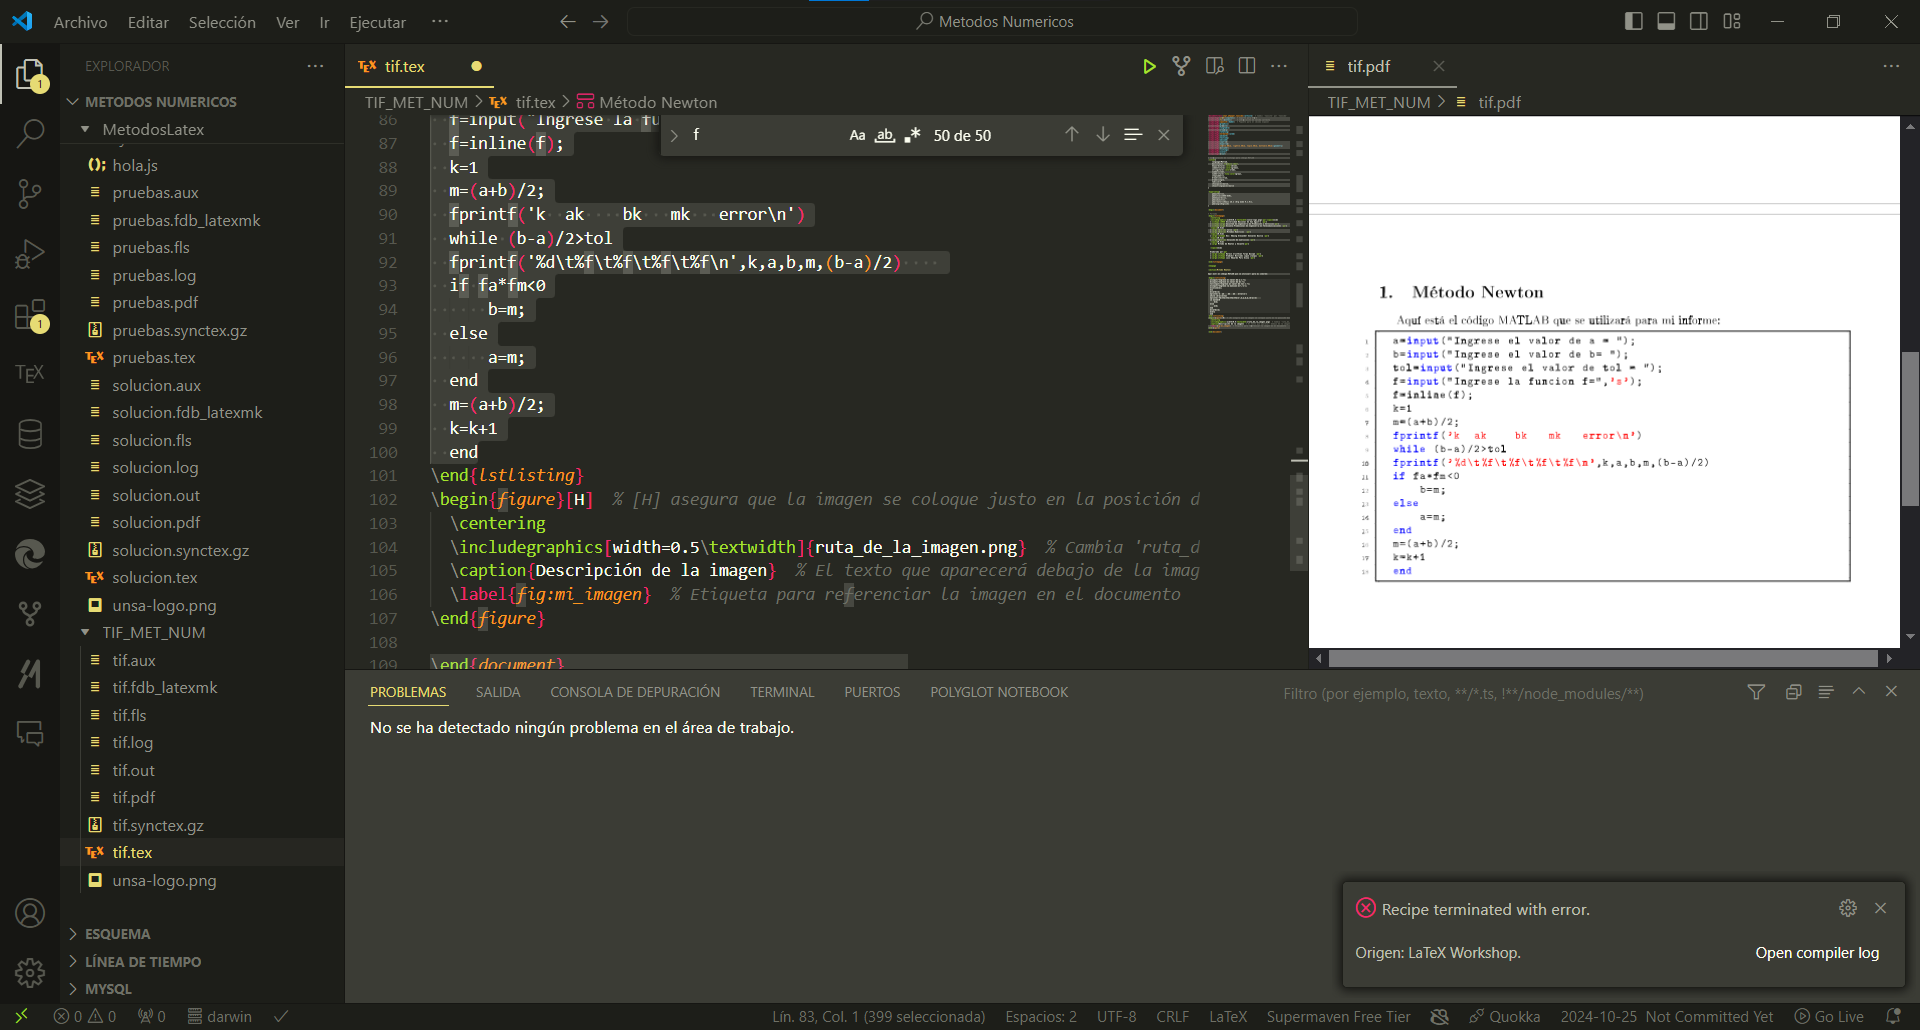
\includegraphics[width=1\textwidth]{1.png}  % Cambia "ruta_de_la_imagen.png" por la ubicación de tu imagen
%  \caption{Descripción de la imagen}  % El texto que aparecerá debajo de la imagen
%  \label{fig:mi_imagen}  % Etiqueta para referenciar la imagen en el documento
%\end{figure}

\end{document}